\documentclass[12pt,a4paper,twoside,nobind]{ociamthesis}

\usepackage[utf8]{inputenc}
\usepackage[T1]{fontenc}
\usepackage[version=4]{mhchem}
\usepackage[position=b]{subcaption}
\usepackage{booktabs, multirow, threeparttable, mathrsfs, xcolor, caption, subcaption, nth, graphicx, svg, floatrow, amsmath, wrapfig, braket,adjustbox}
\usepackage[print-unity-mantissa=false]{siunitx}
% \usepackage[backgroundcolor=white,
%             textsize=footnotesize,textwidth=2cm]{todonotes}
\usepackage[backend=bibtex,style=chem-acs]{biblatex}
\addbibresource{references.bib}
\renewcommand*{\bibfont}{\footnotesize}
%\AtBeginBibliography{\vspace*{-1cm}}

\graphicspath{ {figures/} }
\DeclareGraphicsExtensions{.png}

\newfloatcommand{capbtabbox}{table}[][\FBwidth]
\floatsetup[ffigbox]{capposition=bottom}
\newcommand\MyBox[2][red!70!black]{{%
  \setlength\fboxsep{0pt}\fcolorbox{#1}{white}{#2}}}

\newcommand{\fillcaption}[1]{ %new command with the argument being the text of the caption
	\textbf{Figure \arabic{figure}:} #1 %Makes main figure number, concatenates it to legend
	\addtocounter {figure} {1} %increments main figure count
} 

\setlength{\marginparwidth}{2cm}

\title{Data-driven design of interatomic potentials for metastable chalcogenides}
\author{Joe Morrow}
\college{The Queen's College}
\degree{Transfer of Status Report}
\degreedate{August 2022}

\begin{document}
\setlength{\textbaselineskip}{26pt}
\setlength{\frontmatterbaselineskip}{17pt plus1pt minus1pt}
\setlength{\baselineskip}{\textbaselineskip}
\setlength{\baselineskip}{\singlebaselineskip}
%
% The level that gets a number for ToC:
\setcounter{secnumdepth}{2}
% The level that shows up in the ToC:
\setcounter{tocdepth}{2}
%
\begin{romanpages}
%
\maketitle
%
% \begin{acknowledgements}
%     \input{acknowledgements}
% \end{acknowledgements}
%
\begin{abstract}
  Abstract here
    % \input{abstract}
\end{abstract}
%
%\dominitoc % decide if you want mini ToC (probs not necessary)
%\dominilof
%\dominilot
\flushbottom
\tableofcontents
%
% \listoffigures
%
% \input{abbreviations}
%
\end{romanpages}
%
\chapter{Nature and aims} \label{chap:introduction}
%
%
\section{Introduction}
The research for my DPhil thesis centres around the construction of Machine Learning (ML) interatomic potentials
for use in materials chemistry simulations. ML is a group of techniques for extracting useful information from large datasets
with minimal prior knowledge of any laws underlying the data. 
For our purposes, this data is quantum-mechanical energy and force computations on collections of atoms.
By learning from data, 
an ML potential seeks to accurately approximate the quantum-mechanical potential energy surface (PES) in relevant regions of configuration space.
Since the ML potential function is computationally cheaper to evaluate for a given structure by a factor of around \num{e6},
 near-quantum-mechanical quality can be achieved for simulations on far longer timescales and lengthscales.

 \begin{figure}[ht]
  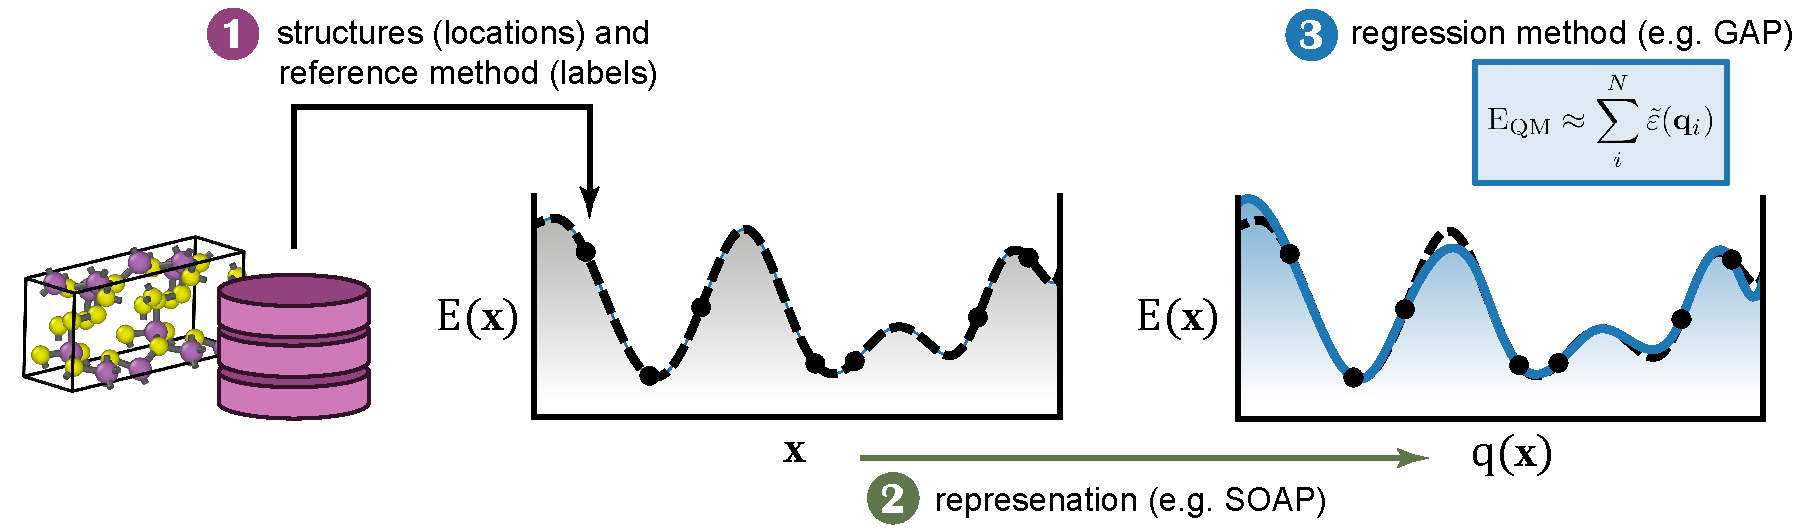
\includegraphics[width=\linewidth]{ML_schematic.pdf}
  \caption{
  Building Machine Learning interatomic potentials. \textbf{1} Building the database, which consists \textbf{2} The representation... \textbf{3} Fitting the data.
  The QM total energy is decomposed into atomic contributions which are a function of the local environment of each atom.
  }
  \label{fig:ML}
\end{figure}

The 3 primary ingredients that go into producing a potential are outlined in Fig.\ \ref{fig:ML}.
Step 1 is building the database:
devising and selecting appropriate structures with enough chemical information to inform the fit,
and calculating the energies and forces of these structures with an accurate reference method (typically DFT).
Step 2 involves encoding the 
local environment of atoms in the database in a mathematical form that is convenient for step 3: the fitting of a flexible function to the reference data.

While I focus primarily on the development of step 1, understanding and practicing steps 2 and 3 are also of critical importance for the performance of the resulting potentials.
There are a number of existing frameworks for 2 and 3, which have been demonstrated to be highly successful in, for example,
describing reactive organic molecules \cite{Ko2021a}, a general purpose model for phosphorus\cite{Deringer2020c}, and  high entropy alloys\cite{Kostiuchenko2019}. 
Two methods of particular interest are the Gaussian Approximation Potential (GAP) framework\cite{Bartok2010}, which employs gaussian process regression as a non-parametric means
to fit the QM data and make predictions on ``unseen'' structures based on the similarity of the new structure to those in the database,
and the Smooth Overlap of Atomic Positions (SOAP) descriptor\cite{Bartok2013}, which represents atomic environments as an overlap integral, hence defining ``similarity''.

\subsection*{Structural databases and GAP-RSS}

ML potentials have few physical constraints beyond rotation, translation, and permutation invariance.
Therefore, far away from regions sampled in the training database, their predictions are quite likely to be unphysical.
In producing many of the successful general-purpose potentials currently available, choosing the strutures to be included in the database was a time-consuming iterative process.
Early versions of the potential were based on snapshots from \textit{ab initio} Molecular Dynamics simulations (AIMD) to sample high temperature liquid and amorphous phases, and
the known crystalline phases of a material with distortions to capture the energy and curvature of minima in the PES. The performance of the resulting potential in predicting the energies
of new structures was then evaluated and any failings remedied using chemical intuition and trial and error, e.g. adding dimer data to capture the core-repulsion at short separations,
or small-scale models of crystalline defects to enable a better description of similar structures. 

% define general purpose

% mention of GAP-RSS for generation of databases, contextualiased with arduous effort of constructing potentials from scratch

% introduction to 

\section{Aims}

\subsection*{Fragment-based random structure searching}

To use 

\subsection*{Modelling \ce{MoS_x}}

\subsection*{Validating ML potentials}


\subsection{Database}

\subsection{Regression}
%
\section{Molybdenum Sulfides}
%
\chapter{Results and Discussion} \label{chap:theory}
%
\section{Indirect learning}

\subsection{Concept}

\begin{figure}[t]
  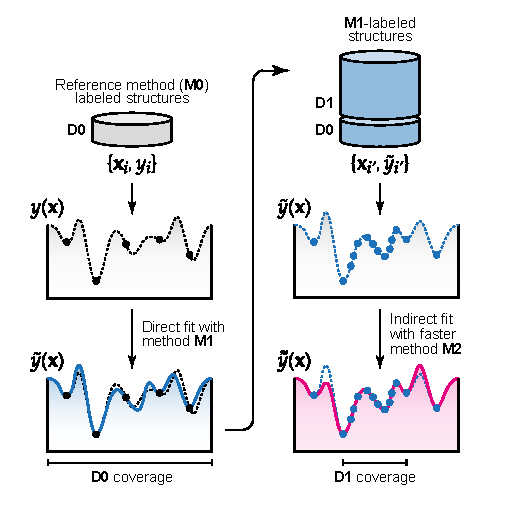
\includegraphics[width=0.5\linewidth]{schematic.pdf}
  \caption{
  Indirect learning of interatomic potentials. 
  \textit{Left:} 
  Conventionally, to fit ML potentials, a potential-energy surface is sampled by reference computations
  for a given number of structures, leading to the dataset \textbf{D0}.
  Fitting with the method \textbf{M1} yields an ML potential model (blue line).
  \textit{Right:}
  We now generate a much larger set of structures using \textbf{M1}, and label them using the same method (not \textbf{M0}!).
  This dataset, \textbf{D1}, covers a narrower structural space, but at more points.
  A second fit is then made with a different ML method, \textbf{M2}.
  }
  \label{fig:schematic}
\end{figure}

\subsection{Application to Silicon}



\subsection{Validation}
\subsubsection{SOAP-based}

\section{Taxonomy of defects in Silicon}

\section{Synthesis and characterisation of \emph{a}-$\ce{MoS3}$}

\section{Random Structure Searching}

%
%
%\begingroup
%\let\clearpage\relax
%\vspace{60pt}
\chapter{Future work}

\section{Further applications of indirect learning}

\section{Modelling of a-$\ce{MoS3}$}
%\endgroup

\clearpage
\section*{Appendix}

%
% \setlength{\baselineskip}{0pt}
% \renewcommand{\abovechapterskip}{\vspace*{-10pt}}
\printbibliography
%
\end{document}